\chapter{Introduction and main concepts}
\setcounter{page}{1}

This course is organised into two big topics which we will go deeper on later. These topics are:
\begin{itemize}
    \item \textbf{Data Mining}, in which we will focus on the \textit{data} side, studying the enabling technologies which have been developed for other purposes, but can positively influence the success of data mining processes;
    \item \textbf{Machine Learning}, in which we will focus on the techniques that support \textit{data–driven decisions}, including learning models and algorithms which allow to extract actionable patterns from data.
\end{itemize}

First of all we have to say that \textit{Data}, \textit{Data Mining} and \textit{Machine Learning} have many differences. While the last two techniques share different concepts, Data exist independently from them, but they need Machine Learning and Data Mining to infer interesting and actionable insights. Especially in the last years these techniques have acquired much more importance with the diffusion of Big Data.

Now we focus on some concepts that represent the basis of all the things that will come after:
\paragraph{Data:} a collection of raw value elements;
\paragraph{Information:} the result of collecting, interpreting and organising data (relationships between items, context and meaning)
\paragraph{Knowledge:} putting together information in order to recognise patterns, according to the needs of the system;
\paragraph{Insight:} all the things that we can infer from knowledge on the basis of what is our goal.

\paragraph{}
When an event in the \textit{real world} changes the state of the enterprise, one of the events below happens:
\begin{itemize}
    \item a \textit{transaction} is executed, i.e. a business event that changes or modifies data stored in an information system (\textit{database});
    \item a \textit{signal} is collected by the infrastructure and stored, which is the reading of a measure provided by a sensor.
\end{itemize}
The concept of \textbf{business} in this case is referred to a \textbf{business process}, i.e. a set of activities that will achieve an \textit{organization goal}, once completed. Outside these two events data can also come from \textit{external subjects}.

\begin{figure}
    \centering
    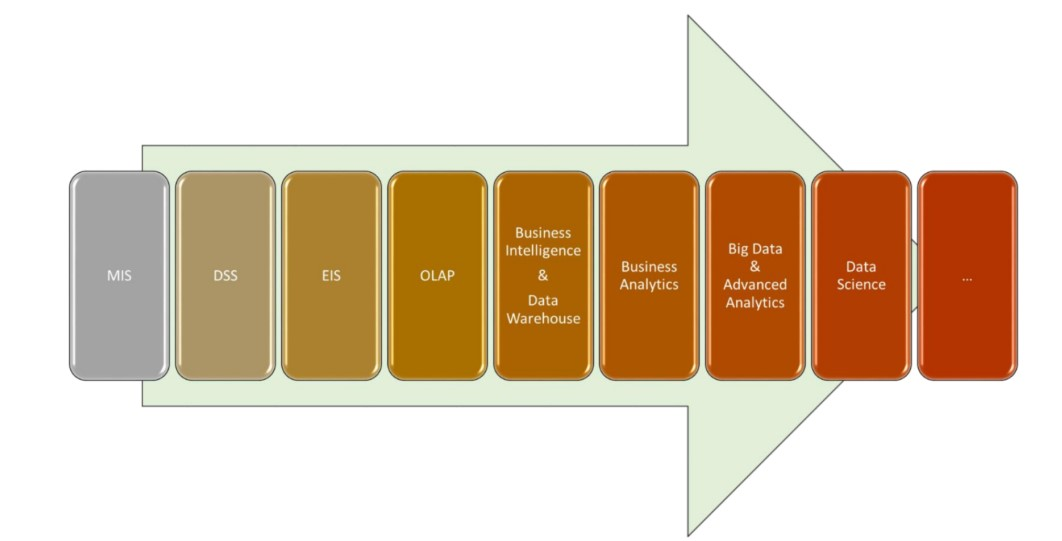
\includegraphics[scale=0.6]{images/increasing_insights.jpg}
    \caption{Increasing insights}
    \label{figInsights}
\end{figure}

\paragraph{OLTP (On-Line Transaction Processing)}
It is a class of software programs capable of supporting transaction-oriented applications and data storage. It is designed to record the daily routine transactions necessary to run the business.

\paragraph{ERP (Enterprise Resource Planning)}
It is a software system that integrates and manages key business processes of all departments within a single software product into a single, unified platform. It operates in or near real time and provide a common database, which supports all the applications.

\paragraph{MIS (Management Information Systems)}
They are standardized reporting systems built on existing OLTP, which work by gathering, processing, managing and delivering important information to support decision-making and management activities within an organization. It is used in working envirnments to generate performance indicators of any type.

\paragraph{DSS (Decision Support Systems)}
They are interactive and computerized information systems that aid individuals and organizations in decision-making by providing data analysis, modeling, and decision-making tools to support a wide range of complex and unstructured decisions.

\paragraph{EIS (Executive Information Systems)}
They are computer-based information systems tailored for senior executives, offering a user-friendly interface that provides consolidated and summarized information from various data sources to support strategic decision-making and organizational performance monitoring.

\paragraph{OLAP (On-Line Analytical Processing)}
It is a computer-based approach that allows users to interact with and analyze data from multiple dimensions, providing a flexible and intuitive way to explore, query, and report on large datasets. It uses algorithms and data structures specifically designed to ease operations like selections, projections, column exchanges, etc.

\paragraph{BI (Business Intelligence)}
It is a set of methodologies, processes, architectures, and technologies that transform raw data into meaningful and useful information used to enable more effective strategic, tactical, and operational insights and decision-making (Forrester Research).
\begin{figure}[ht!]
    \centering
    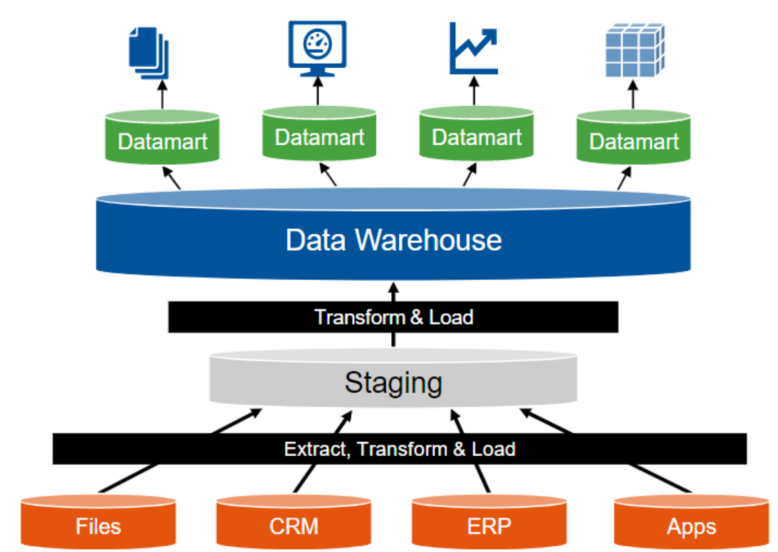
\includegraphics[scale=0.6]{images/BI_architecture.png}
    \caption{BI architecture}
    \label{figBI}
\end{figure}

\paragraph{Analytics}
Structured decisions driven by data and there are different types:
\begin{itemize}
    \item \textbf{descriptive} - understand data 
    \item \textbf{diagnostic} - understand causes
    \item \textbf{predictive} - calculate the most probable value of a variable in a future time, given the history of a set (sequence) of variables
    \item \textbf{prescriptive} - suggest actions to be taken to obtain the desired effect.
\end{itemize}

\paragraph{Cloud Computing}
Cloud computing refers to the delivery of computing services, including storage, processing power, and applications, over the internet.

It is typically categorized into three main service models:
\begin{itemize}
    \item \textbf{Software as a Service (SaaS):} Delivers software applications over the internet on a subscription basis. Users can access and use software applications running on providers' cloud infrastructure.
    \item \textbf{Platform as a Service (PaaS):} Offers a platform that allows users to develop, run, and manage applications without dealing with the complexities of infrastructure. Then applications are deployed on the provider's cloud infrastructure.
    \item \textbf{Infrastructure as a Service (IaaS):} Consumer can use computing resources within provider’s infrastructure upon which they can deploy and run arbitrary software, including OS and applications.
\end{itemize}

\paragraph{Big Data}
Big Data are a collection of data sets so large and/or complex and/or fast changing that they are difficult to process using traditional DBMSs or traditional data processing applications.
\begin{figure}[ht!]
    \centering
    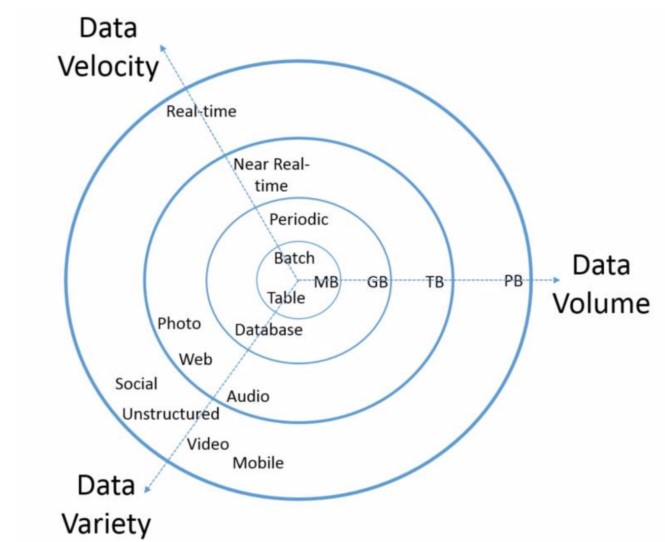
\includegraphics[scale=0.7]{images/BigData_definition.jpg}
\end{figure}

Their taxonomy is divided into data that are:
\begin{itemize}
    \item \textbf{Structured:} relational tables, spreadsheet (or data which could easily fit in them);
    \item \textbf{Unstructured:} does not have an associated data model (video, audio, pictures, etc.);
    \item \textbf{Semi-structured:} there is some structure, perhaps data refer to different structures (XML, JSON, etc.).
\end{itemize}
